\documentclass{ximera}

\usepackage{todonotes}

\newcommand{\RR}{\mathbb R}
\renewcommand{\d}{\,d}
\newcommand{\dd}[2][]{\frac{d #1}{d #2}}
\renewcommand{\l}{\ell}
\newcommand{\ddx}{\frac{d}{dx}}
\newcommand{\dfn}{\textbf}
\newcommand{\eval}[1]{\bigg[ #1 \bigg]}
\renewcommand{\epsilon}{\varepsilon}
\newcommand{\p}[1]{\left(#1\right)}
\newcommand{\br}[1]{\left[#1\right]}
\newcommand{\set}[1]{\left\{#1\right\}}


\let\prelim\lim
\renewcommand{\lim}{\displaystyle\prelim}

\colorlet{textColor}{black} 
\colorlet{background}{white}
\colorlet{penColor}{blue!50!black} % Color of a curve in a plot
\colorlet{penColor2}{red!50!black}% Color of a curve in a plot
\colorlet{penColor3}{red!50!blue} % Color of a curve in a plot
\colorlet{penColor4}{green!50!black} % Color of a curve in a plot
\colorlet{penColor5}{orange!80!black} % Color of a curve in a plot
\colorlet{fill1}{blue!50!black!20} % Color of fill in a plot
\colorlet{fill2}{blue!10} % Color of fill in a plot
\colorlet{fillp}{fill1} % Color of positive area
\colorlet{filln}{red!50!black!20} % Color of negative area
\colorlet{gridColor}{gray!50} % Color of grid in a plot


\newcommand{\fullwidth}{}
\newcommand{\normalwidth}{}



%% makes a snazzy t-chart for evaluating functions
\newenvironment{tchart}{\rowcolors{2}{}{background!90!textColor}\array}{\endarray}


\author{Gregory Hartman \and Matthew Carr}
\license{Creative Commons 3.0 By-NC}
\acknowledgement{https://github.com/APEXCalculus}

\begin{document}
\begin{exercise}

\outcome{Identify when a limit does not exist.}
\outcome{Calculate limits of piecewise functions.}

\tag{limit} 
\tag{piecewise} 
\tag{discontinuous}

  Find 
  \[
  \lim_{x\to 2} f(x)
  \begin{prompt}
  = \answer{\text{DNE}}.
  \end{prompt}
  \]
  where
  \[
  f(x) = \left\{\begin{array}{cl} x+2 & x\leq 2, \\ 3x-5 & x>2. \end{array}\right.
  \]
    \begin{hint}
     Both pieces of $f(x)$, $x+2$, for $x\le2$, and $3x-5$, for $x>2$, are continuous for all $x$. However, for the limit $\lim_{x\to2}f(x)$ to exist, both the left-hand and the right-hand limits of $f(x)$ at $2$ must exist and be equal.
    \end{hint}
     \begin{hint}
    	Take a look at the graph of the function
    \begin{center}
     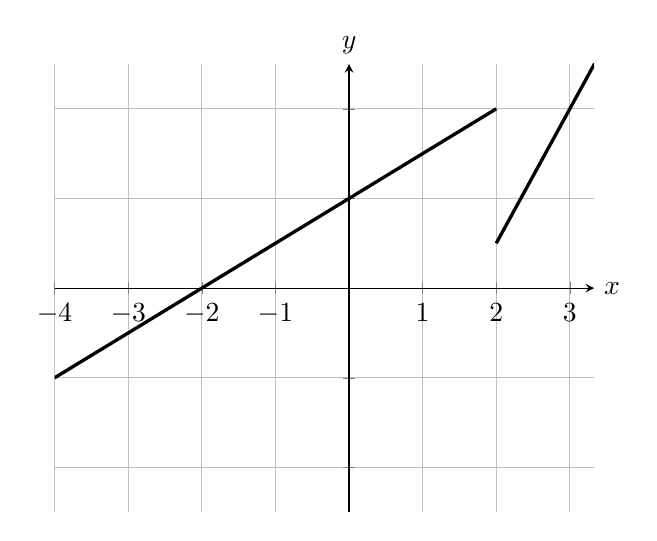
\begin{tikzpicture}
	\begin{axis}
	[ymin=-5,ymax=5, axis lines=center,xlabel=$x$,ylabel=$y$,every axis y 
	label/.style={at=(current axis.above origin),anchor=south},every axis x label/.style={at=(current axis.right of origin),anchor=west},
	domain=-4:4,
	yticklabels={},
	ymajorgrids=true,
	grid = major
	]
	\addplot[domain=-4:2,very thick,smooth,samples=300]
	{2+\x};
	\addplot[domain=2:4,very thick,smooth,samples=300]
	{3*\x-5};
	\end{axis}
       \end{tikzpicture}      
      \end{center} 
    \end{hint}
    \begin{hint}
     Evaluating $\lim_{x\to2^{+}}f(x)$ we see that it is equal to $1$. This follows because, for $x>2$, we are on the piece of $f(x)$ given by $3x-5$ and the limit $\lim_{x\to2}\p{3x-5}=3\cdot\lim_{x\to 2}\p{x}-\lim_{x\to2}\p{5}=1$, certainly. On the other hand, evaluating $\lim_{x\to2^{-}}f(x)$ we see it is equal to $4$. This follows because, for $x\le2$, we are on the piece of $f(x)$ given by $x+2$ and the limit $\lim_{x\to2}\p{x+2}=\lim_{x\to2}\p{x}+\lim_{x\to2}\p{2}=4$, certainly. These are not equal, so $\lim_{x\to 2}f(x)$ does not exist.
    \end{hint} 
\end{exercise}

\end{document}